\section{Resultados}\label{sec:resultados}
\subsection{Soluciones 1D y verificación del código}
Con los datos de la Tabla~\ref{tab:datos}, la Formulación II converge a $Q_1=6.9405\,\Qs$, $Q_2=5.0595\,\Qs$ y $H_J=101.5937$ m ($y_J=1.5937$ m), es decir $\varphi=0.4216$, igual para los cinco ángulos. La Formulación I da, en cambio, un reparto que crece con el ángulo (Tabla~\ref{tab:f1}), con $\lambda=0.75$ y $\mu=0.50$. La diferencia de nivel entre ramales que exigiría el flujo ideal, $(y_1-y_2)/y$, crece de $0.45\pc$ en $30^\circ$ a $15.9\pc$ en $90^\circ$ y $32.3\pc$ en $120^\circ$.

\begin{table}[H]
\centering\small
\caption{Fracción al ramal 2 según la Formulación I.}\label{tab:f1}
\begin{tabular}{lccccc}
\toprule
$\alpha$ ($^\circ$) & 30 & 45 & 60 & 90 & 120\\\midrule
$\varphi_{\mathrm I}=Q_2/Q_0$ & 0.4063 & 0.4353 & 0.4779 & 0.6025 & 0.7845\\\bottomrule
\end{tabular}
\Fuente{Elaboración propia, Newton--Raphson sobre \eqref{eq:f1}.}
\end{table}

La convergencia de Newton--Raphson para la Formulación II se detalla en la Tabla~\ref{tab:iter}: el residuo cae de $1.2\times10^{-1}$ a $2\times10^{-15}$ en cuatro iteraciones, con el comportamiento cuadrático esperado cerca de la raíz. La Figura~\ref{fig:redes} muestra las redes de flujo de la Formulación I para $30^\circ$, $60^\circ$, $90^\circ$ y $120^\circ$ con la geometría de la Fase I del cuaderno ($\lambda=1$, $\mu=0.5$), distinta de la del caso nominal.

\begin{table}[H]
\centering\small
\caption{Historial de Newton--Raphson, Formulación II, caso nominal.}\label{tab:iter}
\begin{tabular}{rrrrr}
\toprule
Iteración & $Q_1$ ($\Qs$) & $Q_2$ ($\Qs$) & $H_J$ (m) & $\|\mathbf F\|_\infty$\\\midrule
0 & 8.823406 & 3.176594 & 101.490000 & $1.247\times10^{-1}$\\
1 & 6.717514 & 5.282486 & 101.568979 & $3.577\times10^{-2}$\\
2 & 6.936867 & 5.063133 & 101.593352 & $5.227\times10^{-4}$\\
3 & 6.940494 & 5.059506 & 101.593677 & $1.326\times10^{-7}$\\
4 & 6.940494 & 5.059506 & 101.593678 & $2.186\times10^{-15}$\\\bottomrule
\end{tabular}
\Fuente{Elaboración propia, \path{codigo/newton_bifurcacion.py}.}
\end{table}

\begin{figure}[H]
\centering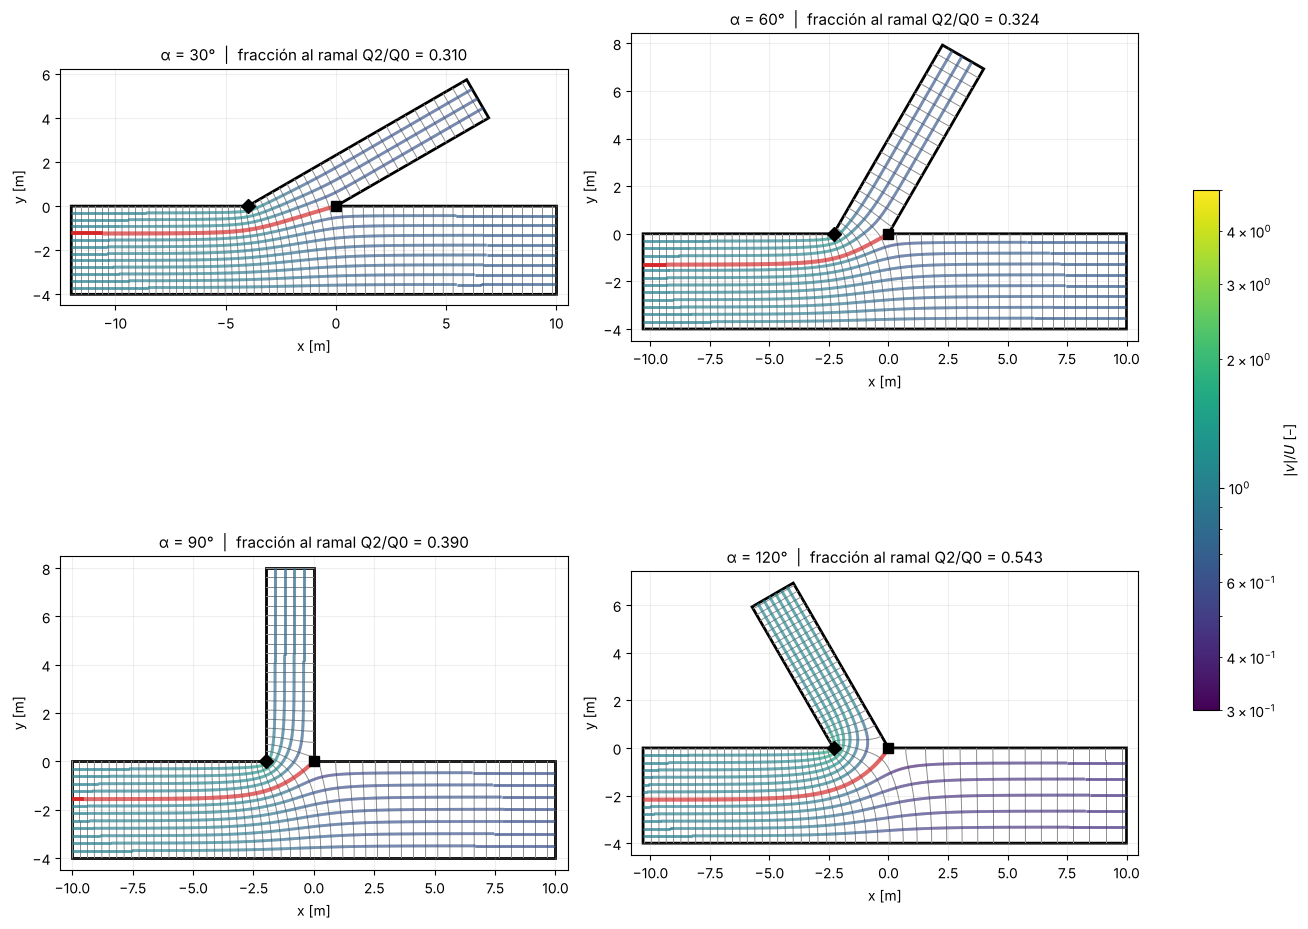
\includegraphics[width=0.92\linewidth]{3.png}
\caption{Redes de flujo de la Formulación I (potencial ideal con tapa rígida) para varios ángulos; la fracción al ramal se indica sobre cada panel.}\label{fig:redes}
\Fuente{Elaboración propia con el cuaderno de la Fase I. Los repartos indicados (0.310, 0.324, 0.390 y 0.543) corresponden a $\lambda=1$ y $\mu=0.5$ y se reprodujeron con Newton--Raphson sobre \eqref{eq:f1}; los de la Tabla~\ref{tab:f1} corresponden a $\lambda=0.75$ y $\mu=0.50$.}
\end{figure}

La Tabla~\ref{tab:verif} resume las pruebas. El benchmark de la red de ocho canales \emph{no se reproduce}: la reconstrucción difiere hasta 33.3\pc (10.5 $\Qs$) de los valores tabulados, y varios calados de esa red se excluyeron por inconsistencias internas. Se reporta como prueba no superada; no se afirma que el código de la red esté validado.

\begin{table}[H]
\centering\small
\caption{Pruebas de verificación.}\label{tab:verif}
\begin{tabular}{>{\raggedright\arraybackslash}p{0.34\linewidth}>{\raggedright\arraybackslash}p{0.34\linewidth}>{\raggedright\arraybackslash}p{0.14\linewidth}}
\toprule
Prueba & Resultado & Estado\\\midrule
Simetría, ramales idénticos & $Q_1=Q_2=2.0000\,\Qs$; error 0 (tolerancia $10^{-10}$) & Cumple\\
Conservación de masa, caso nominal & $Q_1+Q_2-Q_0=0.0000$ & Cumple\\
Hoja 1D del 90° vs. Formulación II & Coincide ($Q_1=6.9405$, $Q_2=5.0595$) & Cumple\\
Hoja de Milne-Thomson vs. Formulación I & Diferencia máx. $|\Delta\varphi|=4.5\times10^{-7}$ & Cumple\\
Red de ocho canales (Chaudhry) & Diferencia relativa máx. 33.3\pc & No cumple\\\bottomrule
\end{tabular}
\end{table}

\subsection{Sensibilidad del reparto}
La Figura~\ref{fig:elast} muestra las elasticidades de $\varphi$ para los 13 parámetros, evaluadas con la configuración simulada de cada ángulo. Dominan los calados de control ($|E|\approx0.8$ a $1.3$, con signo opuesto entre ramales), los anchos de fondo ($|E|\approx0.75$ a $0.96$) y la rugosidad ($|E|\approx0.5$). El caudal total, las longitudes y el coeficiente local tienen efecto pequeño ($|E|\leq0.26$; $|E(K)|\approx0.03$). La incertidumbre postulada produce $\sigma_\varphi=0.031$ a $0.036$ en la aproximación lineal y $0.033$ a $0.037$ en Monte Carlo, con diferencias de $-0.4$ a $+7.6\pc$ entre ambos métodos, de modo que la linealización es adecuada.

\begin{figure}[H]
\centering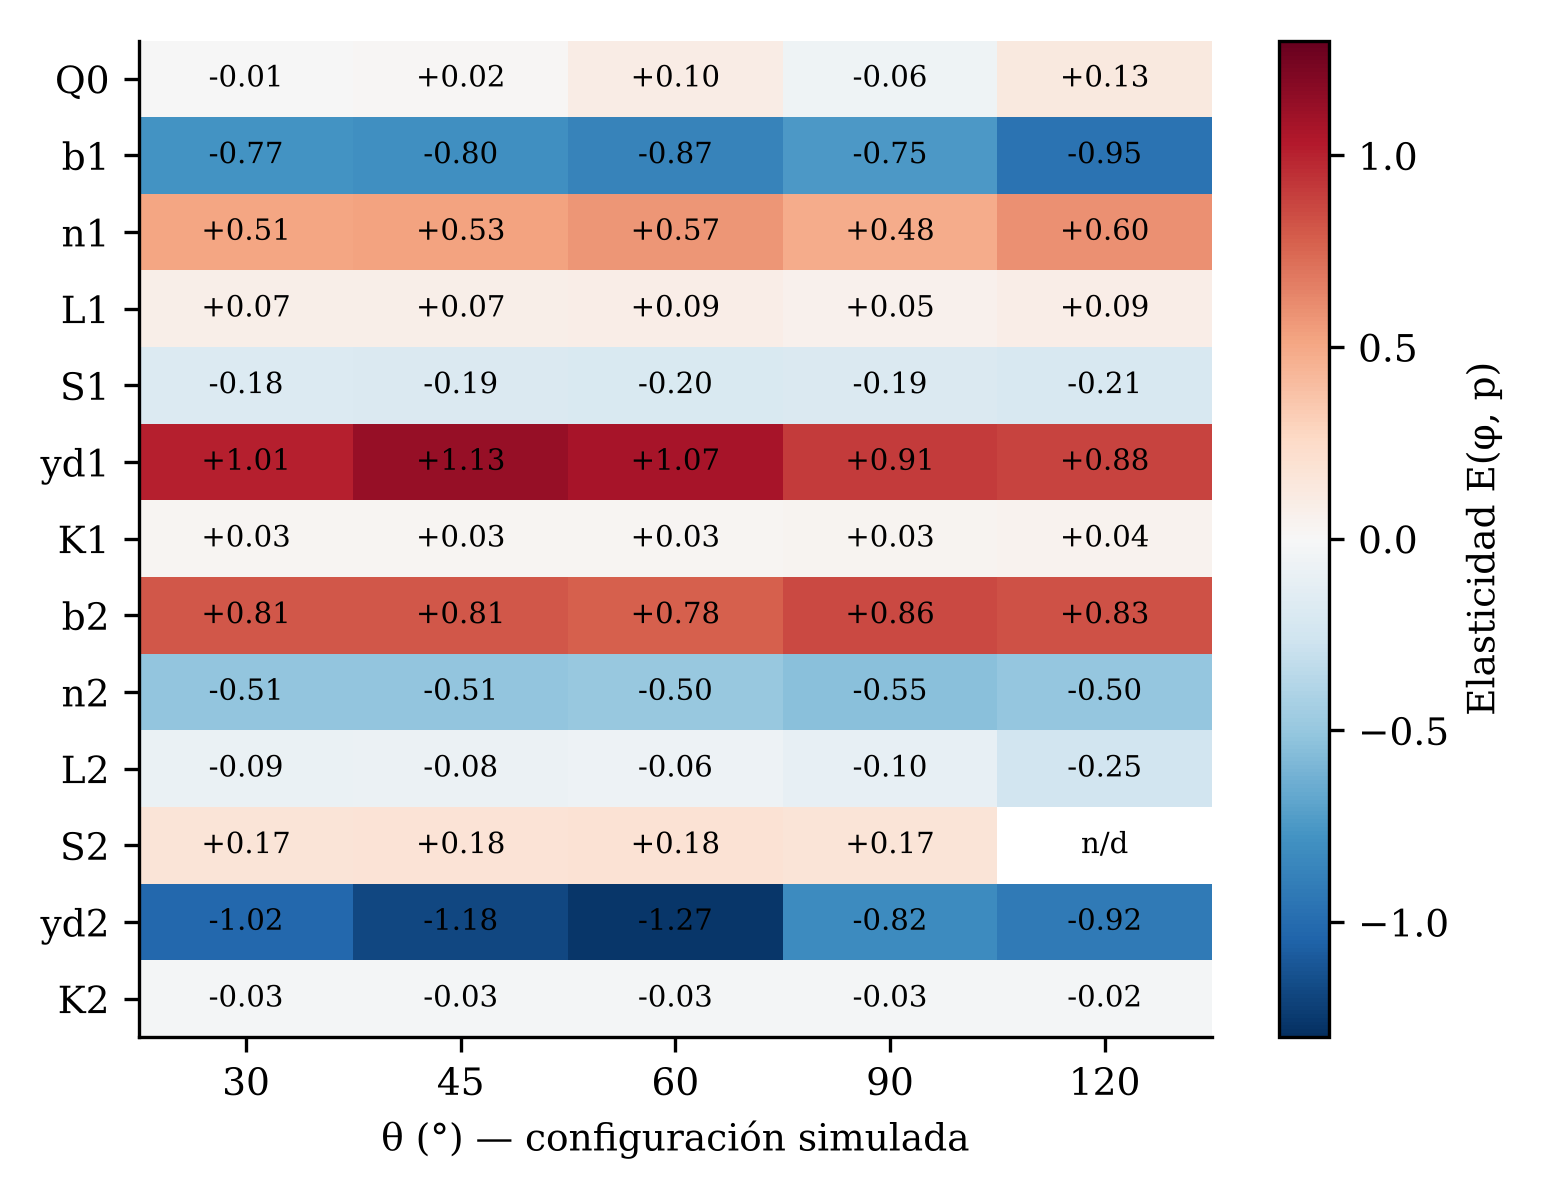
\includegraphics[width=0.62\linewidth]{fig_elasticidad.png}
\caption{Elasticidades de $\varphi$ por ángulo (configuración simulada). Para $120^\circ$, $S_2=0$ y la elasticidad de $S_2$ no está definida.}\label{fig:elast}
\Fuente{Elaboración propia, cuaderno de la Fase IV.}
\end{figure}

\subsection{Resultados del modelo 2D y balance de masa}
La Tabla~\ref{tab:masa} presenta el balance. En los planos disponibles ($45^\circ$ y $90^\circ$) el error del resumen de volúmenes es de $1.2\times10^{-6}\pc$ y $6.3\times10^{-5}\pc$, que coincide con la hoja. En $30^\circ$ el volumen de salida de la hoja supera al de entrada en unos 110 m$^3$ y el error asciende a $0.22\pc$, el único valor no despreciable. En $60^\circ$ la columna de porcentaje repite el valor en m$^3$ (error de hoja); el porcentaje recalculado es $1.3\times10^{-6}\pc$. Los volúmenes de la hoja están redondeados a 10 m$^3$, por lo que errores menores a esa cifra no pueden reconstruirse con ellos.

\begin{table}[H]
\centering\small
\caption{Balance de masa global de las simulaciones 2D.}\label{tab:masa}
\begin{tabular}{rrrrrr}
\toprule
$\theta$ ($^\circ$) & $V_\mathrm{ent}$ (m$^3$) & $V_\mathrm{sal}$ (m$^3$) & $V_\mathrm{alm}$ (m$^3$) & Error (m$^3$) & Error (\%)\\\midrule
30 & 64800 & 64910 & 29.96 & 141.5 & 0.2183\\
45 & 64800 & 64780 & 24.32 & 0.0008 & $1.24\times10^{-6}$\\
60 & 64800 & 64770 & 30.06 & 0.0008 & $1.3\times10^{-6}$\,$^{a}$\\
90 & 64800 & 64780 & 17.91 & 0.0410 & $6.33\times10^{-5}$\\
120 & 64800 & 64770 & 33.23 & 0.0325 & $5.02\times10^{-5}$\\\bottomrule
\end{tabular}
\Nota{$^{a}$ Recalculado; la hoja entregada consigna 0.0008431\pc, igual al valor en m$^3$. Fuente: \path{Balance de masa.xlsx} y resumen de volúmenes de los planos HDF.}
\end{table}

\subsection{Configuración efectivamente simulada}\label{sec:config}
Al reconstruir la configuración de cada corrida a partir de los resultados (rugosidad efectiva, pendiente de fondo y calados de salida) se encuentra que \emph{no coincide con la nominal} en cuatro de los cinco ángulos (Tabla~\ref{tab:config}). El ramal 1 se simuló con $n=0.018$ en $30^\circ$, $45^\circ$ y $60^\circ$ (la nominal es 0.015); en $120^\circ$ el ramal 2 tiene fondo plano ($S_2=0$) en lugar de 0.001; y los calados de salida del 2D (1.28 a 1.53 m) difieren de los nominales (1.60 y 1.40 m) porque las salidas son de calado normal. Estas diferencias proceden de dos defectos del generador de geometría empleado (región de Manning que cubría el ramal 1 para $\theta<90^\circ$ y fondo plano del ramal 2 para $\theta>90^\circ$), ya corregidos en una versión posterior que aún no se ha vuelto a simular. Por esta razón la comparación se hace contra la Formulación II \emph{con la configuración simulada}.

\begin{table}[H]
\centering\small
\caption{Configuración efectivamente simulada frente a la nominal ($n_1=0.015$, $n_2=0.018$, $S_2=0.0010$).}\label{tab:config}
\begin{tabular}{rccccc}
\toprule
$\theta$ ($^\circ$) & $n_1$ & $n_2$ & $S_2$ & $y_{d,1}$ (m) & $y_{d,2}$ (m)\\\midrule
30 & 0.018 & 0.018 & 0.0010 & 1.495 & 1.484\\
45 & 0.018 & 0.018 & 0.0010 & 1.522 & 1.522\\
60 & 0.018 & 0.018 & 0.0010 & 1.496 & 1.530\\
90 & 0.015 & 0.018 & 0.0010 & 1.404 & 1.357\\
120 & 0.015 & 0.018 & 0.0000 & 1.401 & 1.282\\\bottomrule
\end{tabular}
\Fuente{Elaboración propia a partir de los resultados 2D (cuaderno de la Fase IV).}
\end{table}

\subsection{Reparto: contraste 1D--2D}
La Tabla~\ref{tab:reparto} y las Figuras~\ref{fig:reparto} y \ref{fig:errq2} contrastan los predictores. Con los datos nominales, el error de $Q_2$ es $+3.7$, $+6.8$, $+16.9$, $+10.6$ y $+35.4\pc$ (30° a 120°); con la configuración simulada baja a $-2.3$, $-0.2$, $+6.5$, $-2.7$ y $+4.6\pc$, todos aceptables. Con calado normal en las salidas (sin ningún dato del 2D) el error está entre $-8.5$ y $+7.8\pc$ en 30°--90°. La Formulación I produce errores de $-0.1$, $+10.3$, $+32.5$, $+58.0$ y $+152\pc$: acierta en $30^\circ$ y falla de forma creciente con el ángulo, con tendencia opuesta a la del 2D, cuyo reparto tiende a decrecer hasta 0.31 en $120^\circ$. Los sesgos medios de $\Delta\varphi$ son $+0.170$ (I), $+0.051$ (II nominal), $+0.003$ (II simulada) y $-0.007$ (II con calado normal); el error absoluto medio de la II simulada es 0.012, comparable con la incertidumbre de medición del 2D (0.0078).

\begin{table}[H]
\centering\small
\caption{Reparto $\varphi=Q_2/Q_0$ del 2D y de los predictores 1D, con $\varepsilon(Q_2)$ (\%) entre paréntesis.}\label{tab:reparto}
\begin{tabular}{rcccccc}
\toprule
$\theta$ ($^\circ$) & 2D (libro) & I & II nominal & II simulada & II calado normal\\\midrule
30 & 0.4067 & 0.4063 (-0.1) & 0.4216 (+3.7) & 0.3971 (-2.3) & 0.3887 (-4.4)\\
45 & 0.3946 & 0.4353 (+10.3) & 0.4216 (+6.8) & 0.3938 (-0.2) & 0.3887 (-1.5)\\
60 & 0.3606 & 0.4779 (+32.5) & 0.4216 (+16.9) & 0.3839 (+6.5) & 0.3887 (+7.8)\\
90 & 0.3814 & 0.6025 (+58.0) & 0.4216 (+10.6) & 0.3709 (-2.7) & 0.3491 (-8.5)\\
120 & 0.3113 & 0.7845 (+152) & 0.4216 (+35.4) & 0.3255 (+4.6) & n/d\\\bottomrule
\end{tabular}
\Fuente{Elaboración propia (cuaderno de la Fase IV). Incertidumbre de medición del 2D: 0.0078.}
\end{table}

\begin{figure}[H]
\centering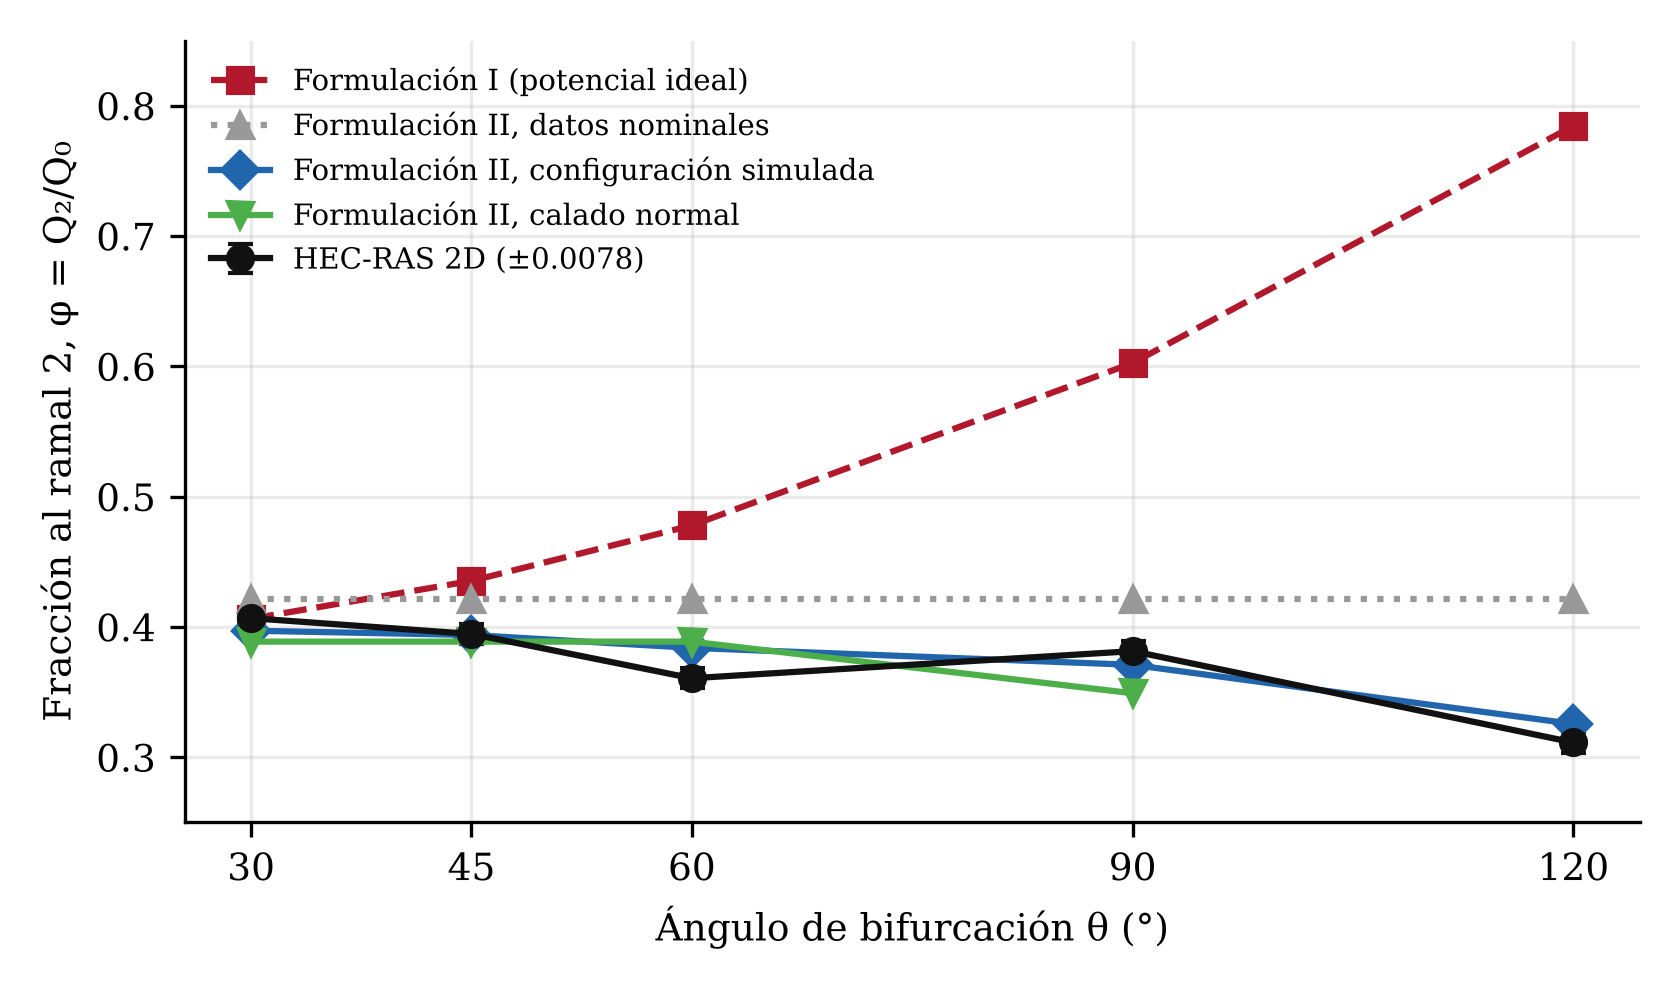
\includegraphics[width=0.74\linewidth]{fig_reparto.png}
\caption{Fracción al ramal 2 en función del ángulo, del 2D y de los predictores.}\label{fig:reparto}
\end{figure}

\begin{figure}[H]
\centering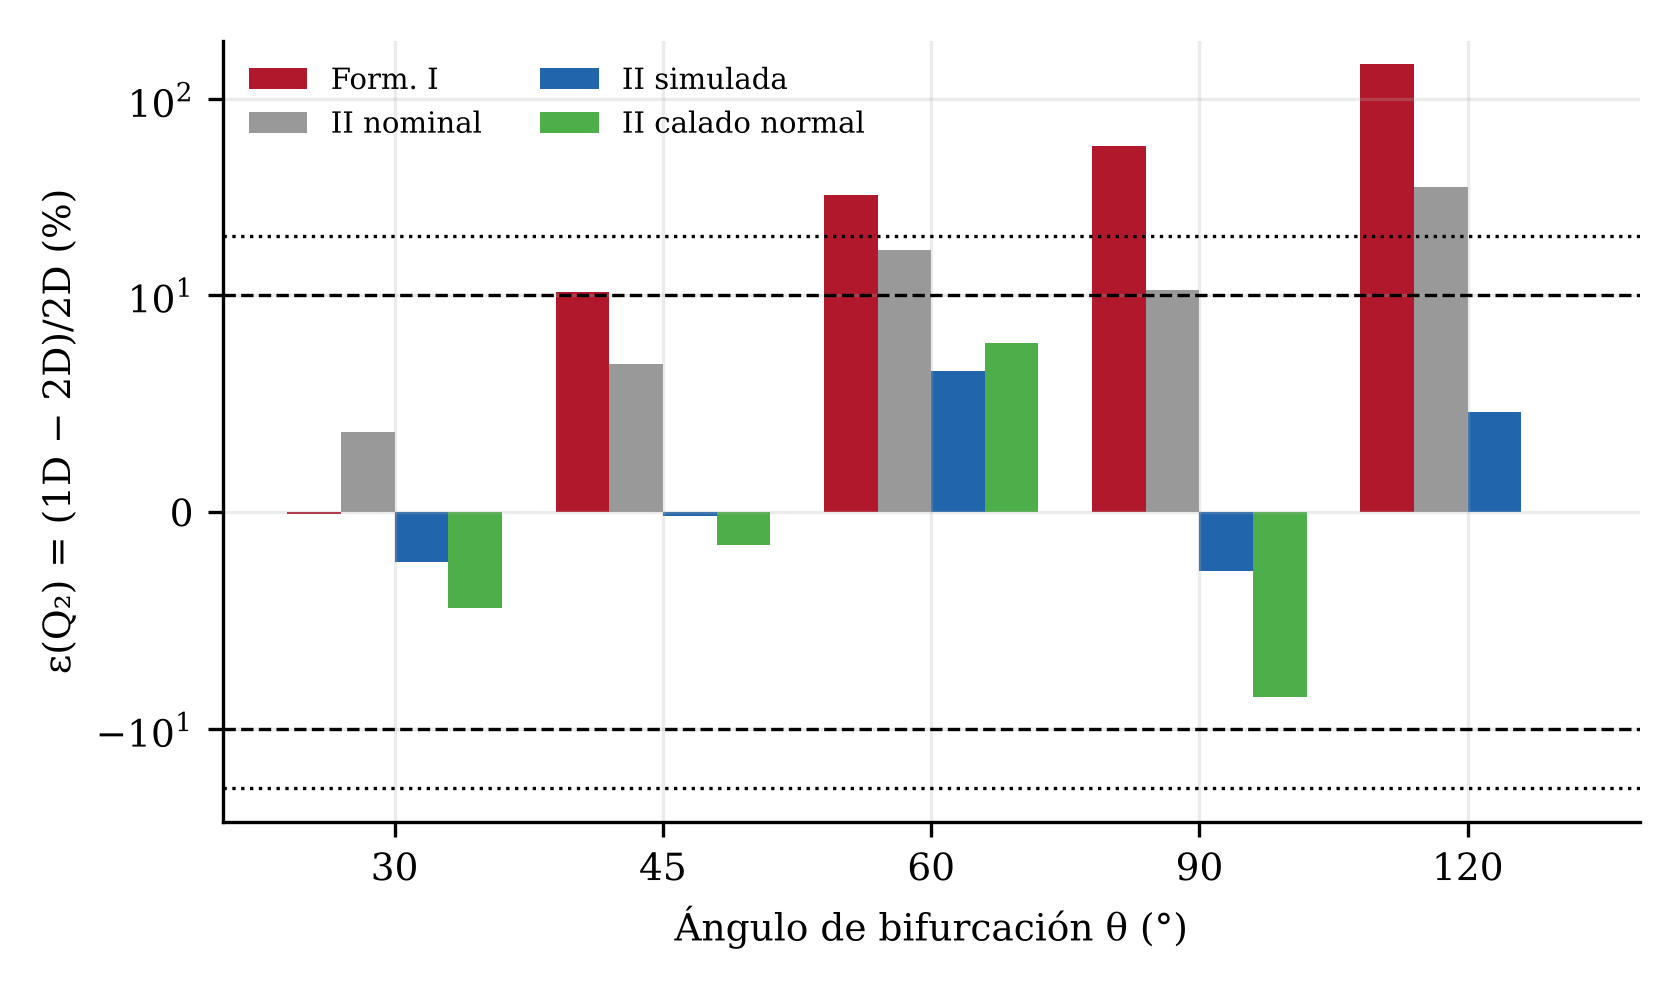
\includegraphics[width=0.74\linewidth]{fig_error_q2.png}
\caption{Error de $Q_2$ respecto del 2D (eje simétrico logarítmico). Líneas discontinuas: $\pm10\pc$; punteadas: $\pm20\pc$.}\label{fig:errq2}
\end{figure}

\subsection{Nivel en la unión}
La Formulación II con la configuración simulada sobrestima el calado en la unión entre $+0.095$ y $+0.128$ m (Figura~\ref{fig:nivel}): marginal en cuatro ángulos y aceptable en $90^\circ$, siempre con el mismo signo. Si en el 1D se aproxima el radio hidráulico por el tirante (pared ancha, como hace el 2D), el error pasa a $-0.053$ a $-0.018$ m. La diferencia que exigiría la Formulación I entre los niveles de los ramales (hasta $+0.485$ m en $120^\circ$) no se observa en el 2D (a lo sumo $0.006$ m).

\begin{figure}[H]
\centering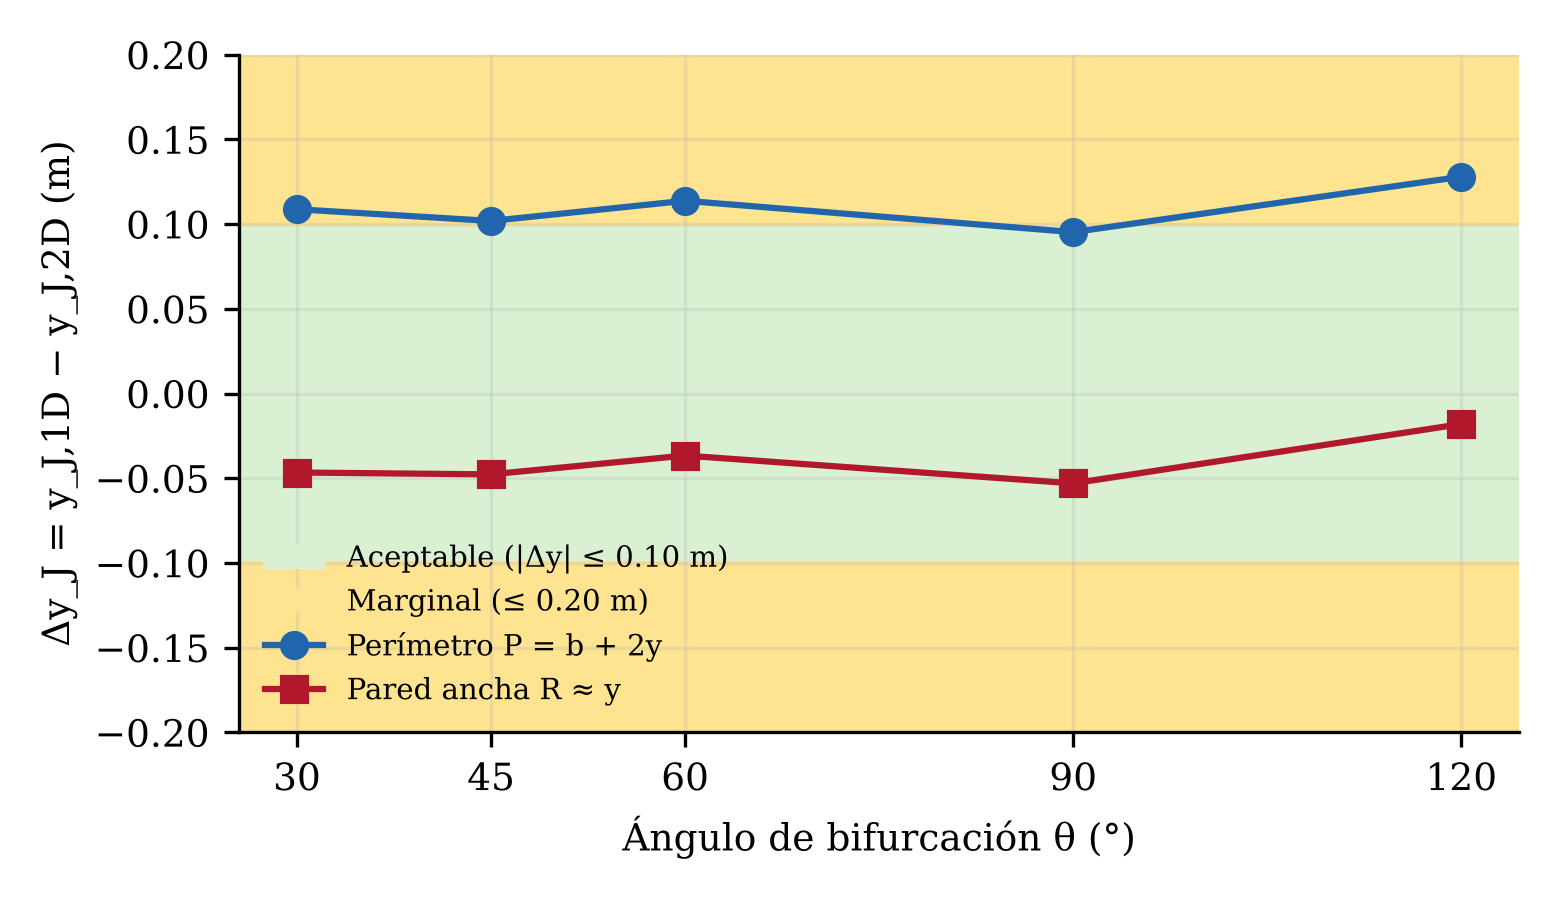
\includegraphics[width=0.68\linewidth]{fig_nivel.png}
\caption{Diferencia de calado en la unión, 1D menos 2D, con dos definiciones del radio hidráulico. Las bandas marcan los umbrales de la Sección~\ref{sec:criterios}.}\label{fig:nivel}
\end{figure}

\subsection{Sesgo, sensibilidad e identificabilidad}
El sesgo de la II simulada es $-0.010$, $-0.001$, $+0.023$, $-0.011$ y $+0.014$ (30° a 120°). Su razón con la incertidumbre paramétrica, $z=B/\sigma_\varphi$, es $-0.27$, $-0.02$, $+0.65$, $-0.32$ y $+0.43$: en los cinco ángulos $|B|\leq2\sigma_\varphi$. Los parámetros que explican el sesgo con el menor desplazamiento son los de rugosidad y los calados de control: en $60^\circ$ bastaría mover $n_1$ en $-0.0019$ ($1.1\sigma$), o $y_{d,2}$ en $+0.073$ m ($1.8\sigma$); el caudal total ($2.2$ a $84\sigma$) y las longitudes ($1.3$ a $48\sigma$) no pueden explicarlo (Tabla~\ref{tab:dp}). La pérdida local $K$ puede cerrar el sesgo con valores de 0.21 a 0.74 (nominal 0.20), pero su efecto sobre $\varphi$ al variar de 0 a 1 es solo $-0.030$ a $-0.045$, apenas 4 a 6 veces la incertidumbre del 2D, de modo que $K$ queda mal identificado.

La descomposición de la diferencia entre la II nominal y el 2D (Figura~\ref{fig:desc}) muestra que corregir la rugosidad y la pendiente simuladas aporta $+0.025$ en $30^\circ$ a $60^\circ$ y $-0.072$ en $120^\circ$, y que imponer los calados de salida del 2D aporta $-0.024$ a $-0.062$; el sesgo restante es de $-0.010$ a $+0.023$.

\begin{table}[H]
\centering\small
\caption{Desplazamiento $|\Delta p^\ast|/\sigma_p$ que cierra el sesgo (valores $\leq2$: explicación plausible).}\label{tab:dp}
\begin{tabular}{lccccc}
\toprule
Parámetro & 30° & 45° & 60° & 90° & 120°\\\midrule
$n_1$ & 0.5 & 0.0 & 1.1 & 0.6 & 0.7\\
$n_2$ & 0.5 & 0.0 & 1.2 & 0.5 & 0.9\\
$y_{d,1}$ & 0.9 & 0.1 & 2.1 & 1.1 & 1.7\\
$y_{d,2}$ & 0.9 & 0.1 & 1.8 & 1.2 & 1.5\\
$b_1$ & 1.6 & 0.1 & 3.5 & 1.9 & 2.3\\
$b_2$ & 1.5 & 0.1 & 3.9 & 1.6 & 2.6\\
$K_1$ & 1.9 & 0.1 & 4.2 & 1.7 & 2.1\\
$K_2$ & 1.9 & 0.2 & 4.7 & 2.2 & 4.2\\
$Q_0$ & 83.7 & 2.2 & 12.1 & 10.1 & 6.9\\
$L_2$ & 13.8 & 1.3 & 47.5 & 13.6 & 8.7\\\bottomrule
\end{tabular}
\Fuente{Elaboración propia (cuaderno de la Fase IV); se omiten $L_1$, $S_1$ y $S_2$.}
\end{table}

\begin{figure}[H]
\centering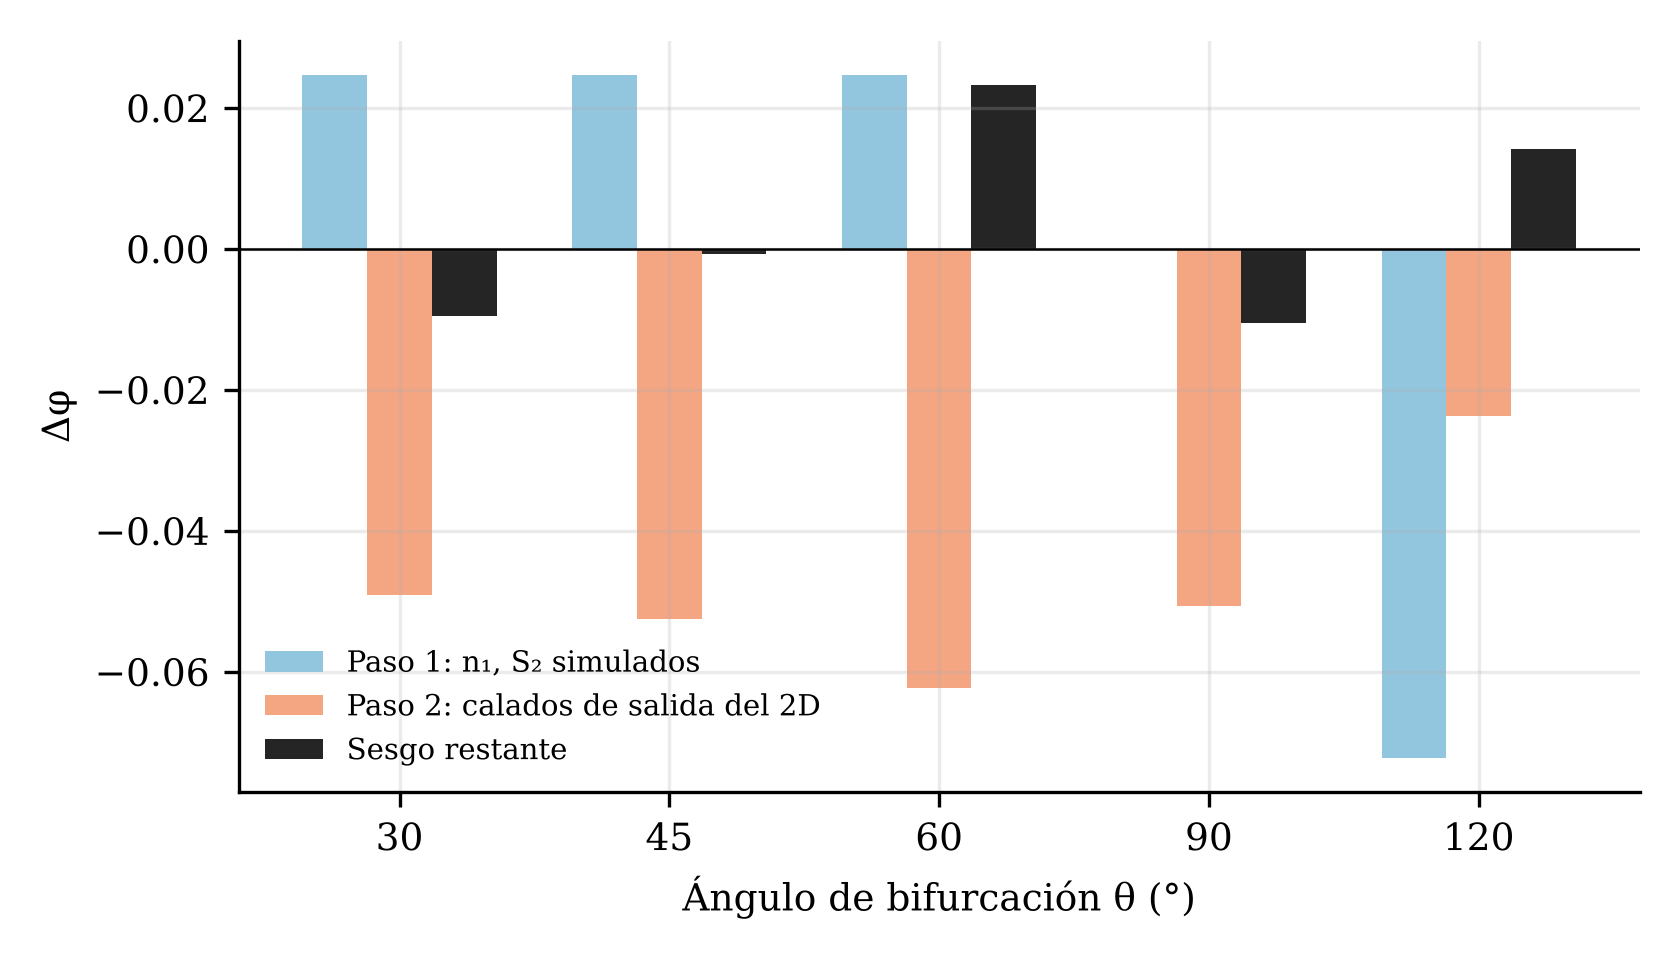
\includegraphics[width=0.74\linewidth]{fig_descomposicion.png}
\caption{Descomposición de $\varphi_{\mathrm{II,nominal}}-\varphi_{2D}$ en el ajuste de la configuración simulada, los calados de salida del 2D y el sesgo restante.}\label{fig:desc}
\end{figure}

\subsection{Evaluación frente a los criterios}
La Tabla~\ref{tab:veredicto} resume la clasificación. El reparto de la Formulación II con la configuración simulada es aceptable en todos los ángulos; el nivel en la unión es marginal en cuatro y aceptable en uno; la Formulación I no es aceptable salvo en $30^\circ$.

\begin{table}[H]
\centering\small
\caption{Clasificación según los criterios de la Sección~\ref{sec:criterios}.}\label{tab:veredicto}
\begin{tabular}{rccc}
\toprule
$\theta$ ($^\circ$) & Formulación I & II (reparto) & II (nivel, $\Delta y_J$)\\\midrule
30 & Aceptable & Aceptable & Marginal ($+0.109$)\\
45 & Marginal & Aceptable & Marginal ($+0.102$)\\
60 & No aceptable & Aceptable & Marginal ($+0.114$)\\
90 & No aceptable & Aceptable & Aceptable ($+0.095$)\\
120 & No aceptable & Aceptable & Marginal ($+0.128$)\\\bottomrule
\end{tabular}
\Nota{La clasificación del reparto de la Formulación II toma el peor de los dos casos (configuración simulada y calado normal).}
\end{table}
